\documentclass[12pt,a4paper]{article}
\usepackage[utf8]{inputenc}
\usepackage[german]{babel}
\usepackage[T1]{fontenc}
\usepackage{amsmath}
\usepackage{amsfonts}
\usepackage{amssymb}
\usepackage{graphicx}
\usepackage[left=2.5cm,right=2.5cm,top=2cm,bottom=2cm]{geometry}
\usepackage{float}
\author{Gruppe C14 \\ Julián Häck, Martin Koytek, Lars Wenning, Erik Zimmermann}
\begin{document}
\begin{figure}[H]
\centering
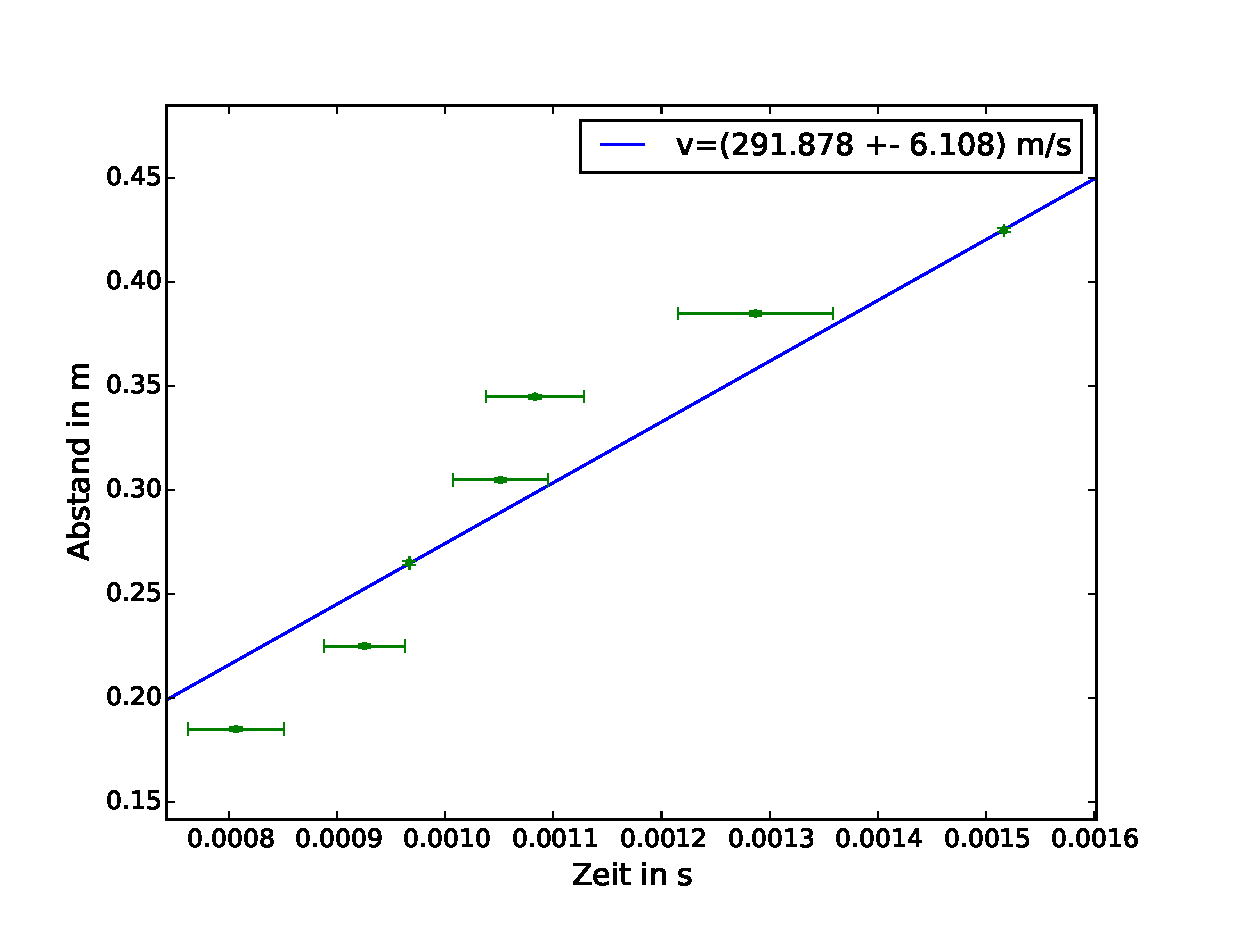
\includegraphics[scale=0.7]{Linreg-cassy-laufzeit.eps}
\caption{Lineare Regression durch die Mittelwerte der Cassy-Messung mit ihren Fehlern}
\end{figure}
\begin{figure}[H]
\centering
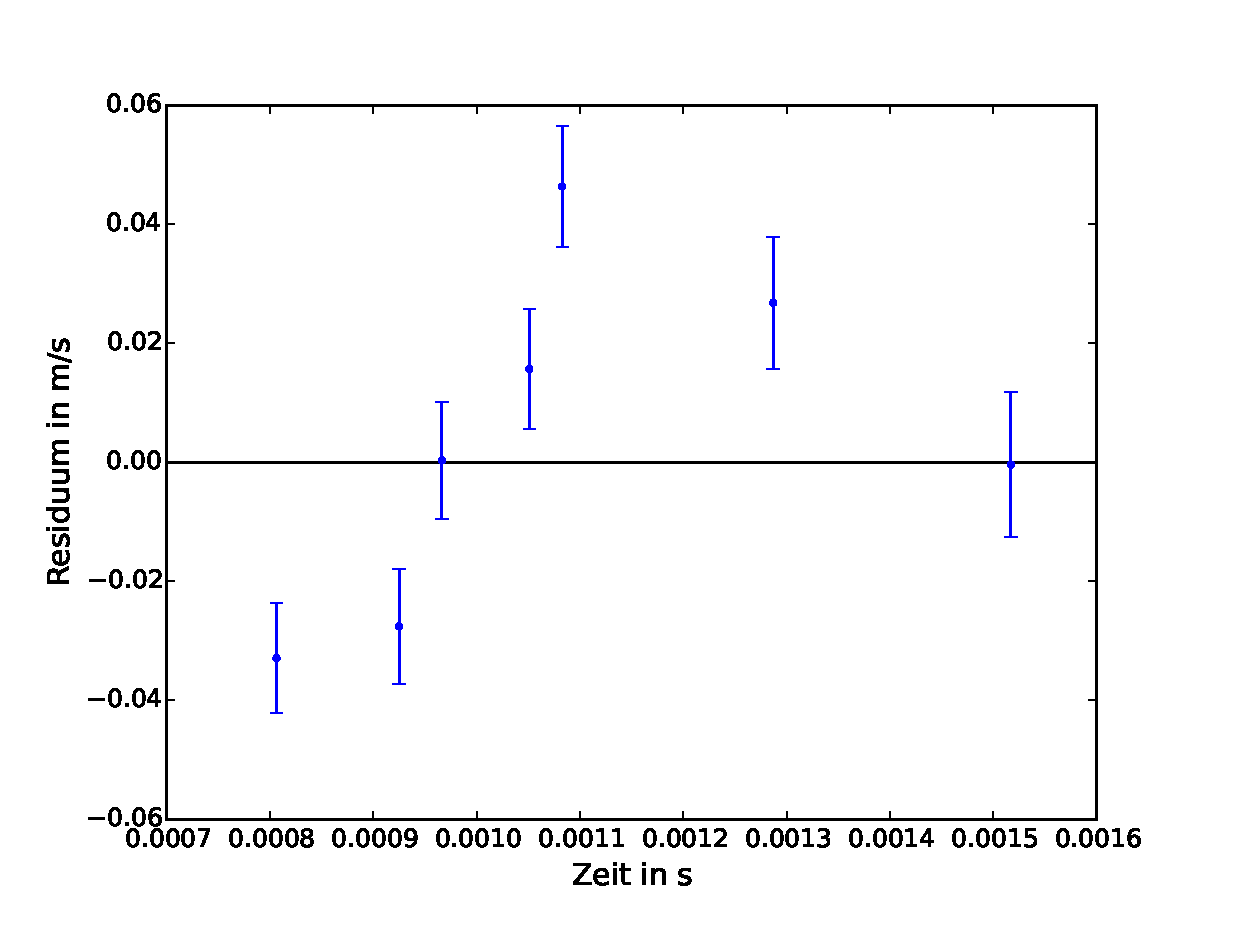
\includegraphics[scale=0.7]{Residuum-cassy-Laufzeit.eps}
\caption{Resiuen des Fits der Cassy-Messung}
\end{figure}
\begin{figure}[H]
\centering
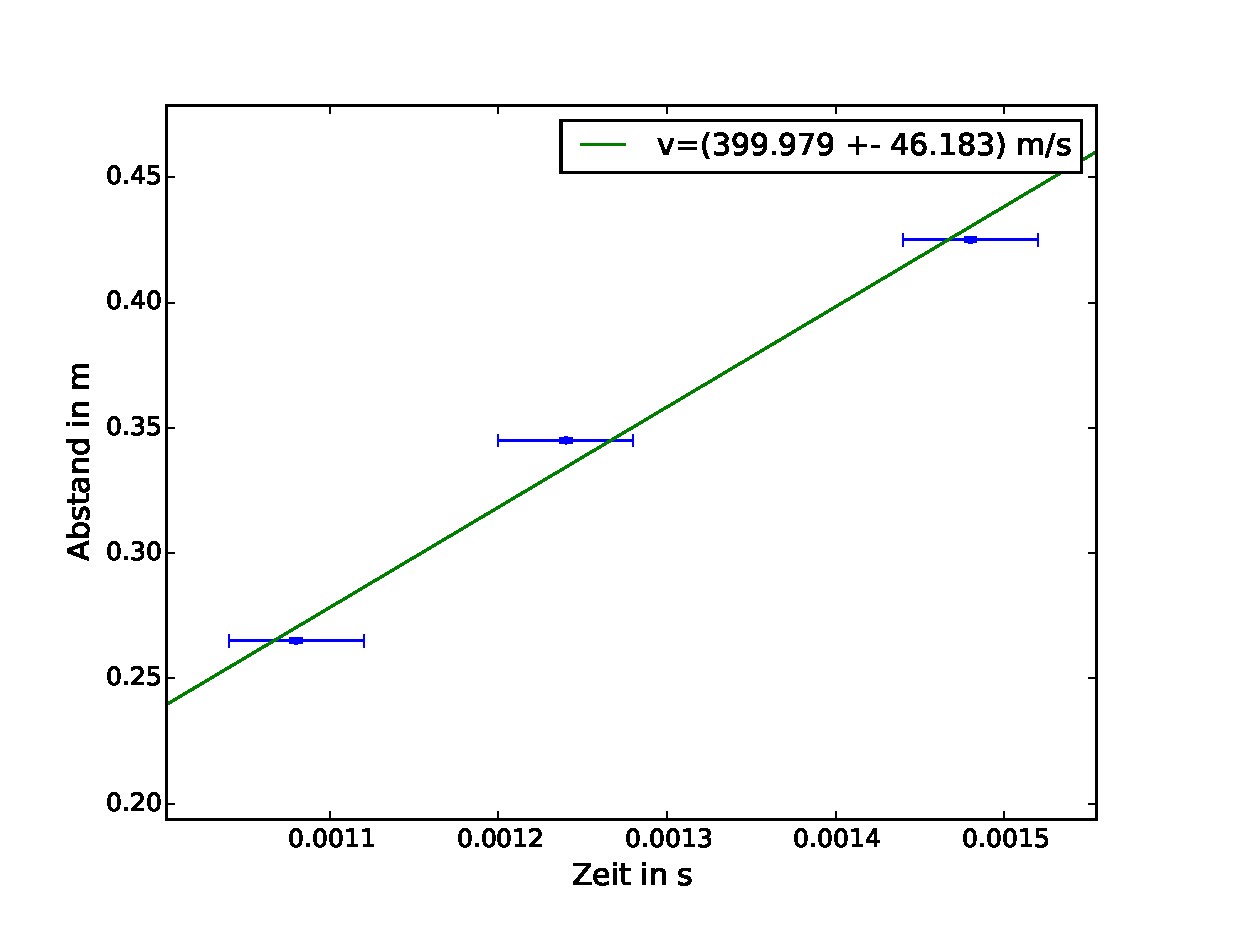
\includegraphics[scale=0.7]{linreg-oszi-laufzeit.eps}
\caption{Lineare Regression der vom Oszilloskop abgelesenen Werte mit ihren Fehlern}
\end{figure}
\begin{figure}[H]
\centering
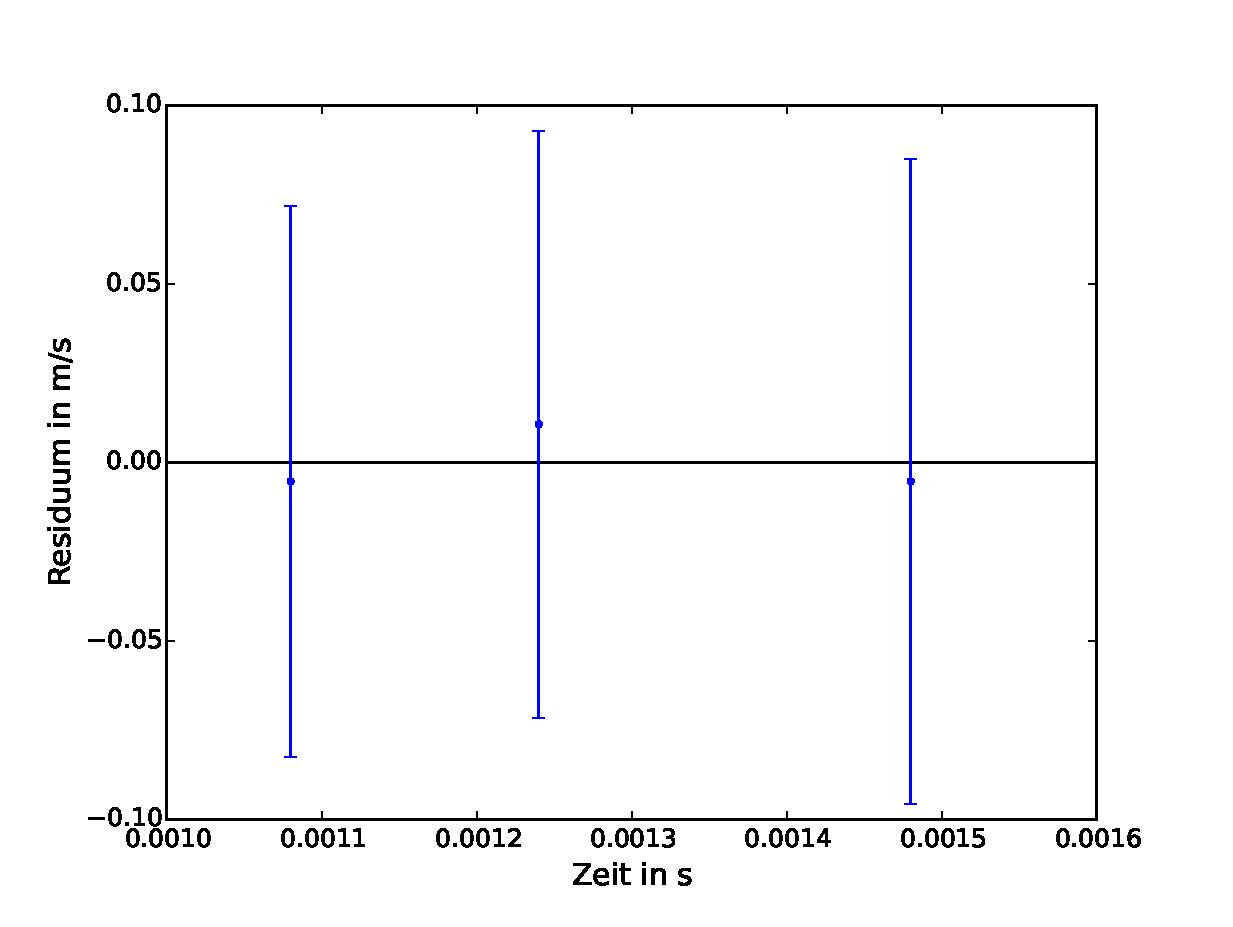
\includegraphics[scale=0.7]{residuum-oszi-laufzeit.eps}
\caption{Residuen des Fits der Oszilloskop-Messung}
\end{figure}
Die x- und y-Fehler der Einzelwerte waren im Pythonscript vertauscht, dadurch kam es zu den großen Fehlerbalken auf der x-Achse. Dies wurde hier korrigiert.
\centering
\begin{tabular}{|c|c|c|}
\hline 
Methode & v in m/s & $\sigma_v$ in m/s \\ 
\hline 
Laufzeit Cassy & 291.8 & 6.1 \\ 
\hline 
Laufzeit Oszilloskop & 400.0 & 46.2 \\ 
\hline 
Variation d. Frequenz & 343.5 & 2.1 \\ 
\hline 
Verm. der stehenden Welle & 352.8 & 4.5 \\ 
\hline 
Literaturwert & 344.98 &  \\ 
\hline 
\end{tabular} 
\end{document}